\documentclass[a4paper,11pt, twoside]{article}
\usepackage{graphicx,listings,float,epstopdf,geometry,amsmath,placeins,caption,subcaption,placeins}
%\usepackage[firstpage]{draftwatermark}
%\SetWatermarkLightness{0.5}
%\SetWatermarkScale{4}
\setcounter{tocdepth}{2}
\usepackage[dutch]{babel}
\usepackage{xspace, color, mdframed}
\usepackage[usenames, dvipsnames]{xcolor}

\geometry{
	includeheadfoot,
	margin=2.54cm
}

% Commando's werkplan
\newcommand{\BS}{BrnStrm}
\newcommand{\ON}{Ori\"entatie}
\newcommand{\MW}{Werkplan}
\newcommand{\MS}{SpelSpec}
\newcommand{\MA}{Spelkeus}
\newcommand{\BO}{Deel. Docu.}
\newcommand{\OC}{Protocol}
\newcommand{\MN}{Impl.Proto.}
\newcommand{\CT}{Proto Test}
\newcommand{\MK}{Klas.diagr.}
\newcommand{\MT}{Taakverdel.}
\newcommand{\IS}{Implement}
\newcommand{\BG}{Handl.}
\newcommand{\AV}{Eind Docu}
\newcommand{\ME}{Mkn.prsnt.}
\newcommand{\EP}{Presenteren}

% Commando's ontwerp
\newcommand{\protoref}{sectie \ref{sec:protocol}}
\newcommand{\bericht}[1]{
    \begin{center}
        \colorbox{YellowGreen!20}{\makebox[\textwidth][c]{{\textsc{#1}}}}
    \end{center}
}
\newcommand{\udp}{\textsc{udp}\xspace}
\newcommand{\tcp}{\textsc{tcp}\xspace}

\begin{document}
	\begin{titlepage}
	\begin{center}
		
		{\Huge Informele Specificatie \\[0.5cm]OGO 2.3 - Multiplayer Game}\\[0.5cm]
		\rule{\linewidth}{0.5mm}\\[0.5cm]
				\bigskip
		\huge \textit{``Grudge of the Oblivious''}
		
		{\Large
		Luca van Ballegooijen, Tim van Dalen, \\
		Carl van Dueren den Hollander, Peter Koymans,\\
		Kay Lukas en Ferry Timmers\\[1cm]
		}
		
		{\large
		OGO 2.3\\
		Groep 3 \\[1cm]
		Faculteit Wiskunde en Informatica\\
		Technische Universiteit Eindhoven\\[1cm]
		}
		
		\begin{abstract}

    In dit document zullen we de kritieke punten bij dit project identificeren. Vervolgens bekijken we de taken die bij dit project een rol spelen. Tenslotte zullen we dit gebruiken om een werkplan voor het project op te stellen.
\end{abstract}


		\vfill

		{\large \today}
	\end{center}
\end{titlepage}

    % Mist nog:
    % - Nummer vak (2IO46)
    % - Identiteitsnummers groepsleden
    % -	Naam tutor (Mels van Broekhoven)
    % Schieten veranderd.

	\tableofcontents
	\newpage

	\section{Lijst symbolen en afkortingen}
    % Verklaring van alle gebruikte symbolen	
    \newpage

    \section{Summary}
    % Engelstalige samenvatting

    \section{Inleiding}
    Informatici in de hedendaagse wereld komen vaak in aanraking met het ontwerpen van complexe programma's. Complexe programma's hebben vaak ook een netwerk aspect en een grafische aspect. Zelfs bij technische programma's, die vaak minder grafisch intensief zijn, als matlab worden al deze aspecten verenigd. Dit drukt de noodzaak uit dat elke informaticus basiskennis heeft van computergrafiek, computernetwerken en het ontwerpen van complexe programma's. Al deze aspecten worden verenigd in dit project: \textsc{ogo} 2.3 - Nethunt. Dit document ligt ... INSERT MORE

Voor dit project werd ons gevraagd om een interactief, gedistribueerd 3D-spel te ontwikkelen. Dit houdt in dat elk speler lokaal dezelfde spelsituatie heeft, en deze op het scherm van de speler worden afgebeeld. Natuurlijk kan de afbeelding op het scherm verschillen per speler. Een andere eis was dat er voedsel aanwezig moet zijn. E\'en van de randvoorwaarden was dat elke speler ... INSERT MORE
    % Probleem- of vraagstelling
    % Opbouw

    \documentclass[a4paper,11pt]{article}
\usepackage{graphicx,listings,float,geometry}
%\usepackage[firstpage]{draftwatermark}
%\SetWatermarkLightness{0.5}
%\SetWatermarkScale{4}
\setcounter{tocdepth}{2}

\geometry{
	includeheadfoot,
	margin=2.54cm
}

\newcommand{\BS}{BrnStrm}
\newcommand{\ON}{Ori\"entatie}
\newcommand{\MW}{Werkplan}
\newcommand{\MS}{SpelSpec}
\newcommand{\MA}{Spelkeus}
\newcommand{\BO}{Deel. Docu.}
\newcommand{\OC}{Protocol}
\newcommand{\MN}{Impl.Proto.}
\newcommand{\CT}{Proto Test}
\newcommand{\MK}{Klas.diagr.}
\newcommand{\MT}{Taakverdel.}
\newcommand{\IS}{Implement}
\newcommand{\BG}{Handl.}
\newcommand{\AV}{Eind Docu}
\newcommand{\ME}{Mkn.prsnt.}
\newcommand{\EP}{Presenteren}

\usepackage[dutch]{babel}
\newenvironment{widepar}%
  {\setlength{\leftskip}{-\marginparsep}\addtolength{\leftskip}{-\marginparwidth}}{\par}

\begin{document}
	\begin{titlepage}
	\begin{center}
		
		{\Huge Informele Specificatie \\[0.5cm]OGO 2.3 - Multiplayer Game}\\[0.5cm]
		\rule{\linewidth}{0.5mm}\\[0.5cm]
				\bigskip
		\huge \textit{``Grudge of the Oblivious''}
		
		{\Large
		Luca van Ballegooijen, Tim van Dalen, \\
		Carl van Dueren den Hollander, Peter Koymans,\\
		Kay Lukas en Ferry Timmers\\[1cm]
		}
		
		{\large
		OGO 2.3\\
		Groep 3 \\[1cm]
		Faculteit Wiskunde en Informatica\\
		Technische Universiteit Eindhoven\\[1cm]
		}
		
		\begin{abstract}

    In dit document zullen we de kritieke punten bij dit project identificeren. Vervolgens bekijken we de taken die bij dit project een rol spelen. Tenslotte zullen we dit gebruiken om een werkplan voor het project op te stellen.
\end{abstract}


		\vfill

		{\large \today}
	\end{center}
\end{titlepage}

	
	\tableofcontents
	\newpage

	\section{Kritieke punten}
    We beginnen met het identificeren van de kritieke punten. Met deze kritieke punten kan dan later rekening worden gehouden in het werkplan. De voornaamste problemen tijdens dit project zijn:
    \begin{enumerate}
    \item[(a)] Het grootste probleem voor het maken van het programma is het netwerk aspect. Hierbij identificeren we twee mogelijke obstakels. Ten eerste moet het mogelijk zijn om elkaar te kunnen vinden over het netwerk. Dit is zeker geen triviale taak. Ten tweede geldt dat gedurende het spel alle machines op gelijke voet staan. Er mag dus geen server worden gebruikt, wat het ontwerp van het spel moeilijker maakt.
    \item[(b)] Een ander groot gevaar is complexiteit. Bij het ontwikkelen van een spel kan men al snel uit enthousiasme hoge verwachtingen krijgen en hoge eisen stellen. Deze overmaat aan eisen kan later te veel werk blijken.
    \item[(c)] Een laatste hindernis is het gedistribueerde aspect met name in conflictsituaties. Een goed voorbeeld hiervan is als twee spelers op hetzelfde moment voedsel proberen te pakken. Als hier geen rekening mee wordt gehouden, kan dit leiden tot een inconsistente toestand. Zo zou het kunnen gebeuren dat beide spelers \'e\'en voedsel object verkrijgen, wat ongewenst is.
    \end{enumerate}

    In ons werkplan proberen we al vroeg mogelijk om met deze kritieke punten rekening te houden. Aangezien we (a) als het voornaamste probleem beschouwen, zullen we in week 1 ons al ori\"enteren op het probleem. We zullen vooral kijken naar de mogelijkheden voor broadcast. Probleem (b) pakken we aan door te beginnen met een kleine hoeveelheid aan eisen voor het spel. Later kan het spel dan worden uitgebreid. In verband met probleem (c) is het slim om al snel te beginnen met het ontwerp van het communicatieprotocol. Er wordt pas begonnen aan dit aspect van het programma zodra het communicatieprotocol is voltooid. Na het voltooien van het communicatieprotocol zal dit uitgebreid worden getest.

    \section{De taken}
    Nu we de mogelijke problemen hebben bekeken, zijn we klaar om een lijst met taken op te stellen met afkortingen. De genoemde taken staan ruwweg in chronologische volgorde:
    \begin{enumerate}
    \item[-] Brainstormen over spelidee (\emph{\BS}).
    \item[-] Ori\"entatie op netwerk aspect door het maken van eenvoudig chat programma (\emph{\ON}).
    \item[-] Maken werkplan met taakverdeling (\emph{\MW}).
    \item[-] Maken spelspecificatie en gebruikershandleiding (\emph{\MS}).
    \item[-] Maken alternatieven en motivering van spelkeuze (\emph{\MA}).
    \item[-] Beschrijving onderdelen en onderlinge samenhang (\emph{\BO}).
    \item[-] Ontwerpen communicatieprotocol (\emph{\OC}).
    \item[-] Maken onderliggende netwerkcommunicatie (\emph{\MN}).
    \item[-] Communicatieprotocol testen (\emph{\CT}).
    \item[-] Maken klassendiagram (\emph{\MK}).
    \item[-] Maken taakverdeling voor implementatie (\emph{\MT}).
    \item[-] Implementatie spel (\emph{\IS}).
    \item[-] Bijwerken gebruikershandleiding, validatie aannames en motivering implementatie (\emph{\BG}).
    \item[-] Afronden verslag (\emph{\AV}).
    \item[-] Maken eindpresentatie (\emph{\ME}).
    \item[-] Eindpresentatie (\emph{\EP}).
    \end{enumerate}

    \section{Het werkplan}
    Als laatste moeten de taken nog over de personen worden verdeeld. Hierbij zullen we taken proberen te rouleren zodanig dat iedereen zowel taken heeft voor programmeren als documenteren. Aangezien wij allemaal zowel ervaring hebben met programmeren als met documenteren, zullen we bij de taakverdeling geen speciale rekening houden met de koppels (bijvoorbeeld relatief goede programmeurs bij relatief zwakke programmeurs).

    We hebben besloten om drie belangrijke zaken samen te doen. Ten eerste is het natuurlijk erg logisch dat het brainstormen samen gebeurt. Hierdoor weten we allemaal in welke richting het spel zal gaan, wat bij alle volgende stappen van belang zal zijn. Ten tweede wordt het communicatieprotocol samen ontworpen. Dit heeft tot doel zodat iedereen het communicatieprotocol goed snapt, zodat iedereen hiermee overweg kan met de implementatie. Ten derde wordt het testen van het communicatieprotocol samen gedaan. De voornaamste reden hiervoor is vanwege de grote diversiteit aan operating systemen in onze groep, wat eventueel problemen kan geven bij de implementatie. We zijn nu klaar om het volledige werkplan te geven, we gebruiken hierbij de eerder gegeven afkortingen. De deadlines staan op een aparte regel en zijn schuin gedrukt:
        \begin{figure}[H]
        \small
        \centering
        \begin{tabular}{| l | l | l | l | l | l | l |}
        \hline
        Week & Carl & Ferry & Kay & Luca & Peter & Tim \\ \hline
        Week 1 24-04-2012 & \BS & \BS & \BS & \BS & \BS & \BS \\ \hline
        Week 1 25-04-2012 & \ON & \ON & \ON & \ON & \MW & \ON \\ \hline
        Week 1 26-04-2012 & \ON & \ON & \ON & \ON & \MW & \ON \\ \hline
        Week 2 01-05-2012 & \MS & \MA & \MA & \MS & \MA & \MS \\ \hline
        Week 2 02-05-2012 & \MS & \MA & \MA & \MS & \MA & \MS \\ \hline
        Week 2 03-05-2012 & \MS & \MA & \MA & \MS & \MA & \MS \\ \hline
        Week 2 04-05-2012 & \multicolumn{6}{|c|}{\emph{Deadline ori\"entatiefase}} \\ \hline
        Week 3 08-05-2012 & \MS & \MA & \MA & \MS & \MA & \MS \\ \hline
        Week 3 09-05-2012 & \MS & \MA & \MA & \MS & \MA & \MS \\ \hline
        Week 3 10-05-2012 & \MS & \MA & \MA & \MS & \MA & \MS \\ \hline
        Week 4 15-05-2012 & \OC & \OC & \OC & \OC & \OC & \OC \\ \hline
        Week 4 16-05-2012 & \OC & \OC & \OC & \OC & \OC & \OC \\ \hline
        Week 4 16-05-2012 & \multicolumn{6}{|c|}{\emph{Deadline specificatiefase}} \\ \hline
        Week 5 22-05-2012 & \BO & \MN & \MK & \MK & \BO & \MN \\ \hline
        Week 5 23-05-2012 & \BO & \MN & \MK & \MK & \BO & \MN \\ \hline
        Week 5 24-05-2012 & \BO & \MN & \MK & \MT & \BO & \MN \\ \hline
        Week 6 30-05-2012 & \BO & \MN & \MK & \MT & \BO & \MN \\ \hline
        Week 6 31-05-2012 & \CT & \CT & \CT & \CT & \CT & \CT \\ \hline
        Week 6 01-06-2012 & \multicolumn{6}{|c|}{\emph{Deadline ontwerpfase}} \\ \hline
        Week 7 05-06-2012 & \IS & \IS & \IS & \IS & \IS & \IS \\ \hline
        Week 7 06-06-2012 & \IS & \IS & \IS & \IS & \IS & \IS \\ \hline
        Week 7 07-06-2012 & \IS & \IS & \IS & \IS & \IS & \IS \\ \hline
        Week 8 12-06-2012 & \BG & \IS & \IS & \IS & \IS & \BG \\ \hline
        Week 8 13-06-2012 & \BG & \IS & \IS & \IS & \IS & \BG \\ \hline
        Week 8 14-06-2012 & \BG & \IS & \IS & \IS & \IS & \BG \\ \hline
        Week 8 14-06-2012 & \multicolumn{6}{|c|}{\emph{Deadline implementatiefase eerste versie}} \\ \hline
        Week 9 19-06-2012 & \AV & \AV & \ME & \AV & \AV & \ME \\ \hline
        Week 9 20-06-2012 & \AV & \AV & \ME & \AV & \AV & \ME \\ \hline
        Week 9 21-06-2012 & \EP & \EP & \EP & \EP & \EP & \EP \\ \hline
        Week 9 22-06-2012 & \multicolumn{6}{|c|}{\emph{Deadline verslag}} \\ \hline
        \end{tabular}
        \caption{Gedetailleerde taakverdeling per dag}
        \label{tab:planning}
    \end{figure}

    Zoals in de tabel is te zien, zijn er ongeveer twee weken om aan de implementatie te werken. Het idee is dat dan een groot deel van het netwerk aspect, wat het grootste risico heeft om uit te lopen, daarvoor al af te hebben om dit op te vangen. Bij de implementatie moet dus vooral aandacht worden besteed aan het modelleren van de scene en het maken van het spel. Een gedetailleerde beschrijving voor de taakverdeling wordt pas in week 6 gemaakt, aangezien daarvoor een deel van de ontwerpfase al moet zijn voltooid.
\end{document}

    % REFERENCE optioneel
        \section{Specificatie}
    Het spel, \emph{Grudge of the Oblivious} (\textsc{goto}), dat wij van plan zijn om te ontwerpen, is een combinatie van een FPS spel en een RTS spel. Dit betekent dat de gebruiker van het spel zowel kan schieten als gebouwen kan bouwen. We beschrijven in appendix \ref{app:alternatieven} de door ons geanalyseerde alternatieve ontwerpen voor een spel. In appendix \ref{app:motivering} motiveren wij de keuze voor ons spel. Op basis van deze specificatie is er een gebruikershandleiding gemaakt. De gebruikershandleiding is te vinden in appendix \ref{app:handleiding}.

    Het spel speelt zich af in een oorlog tussen twee rivaliserende robot-bendes. Deze robot-bendes hebben een corresponderend commandocentrum. In het spel kan een robot-bende als team gezien worden, een dergelijk team bestaat uit meerdere robots en spelers. Elke speler bestuurt \'e\'en robot. Er zijn evenveel robots als spelers.

    Het doel van het spel is om het commandocentrum van de tegenstander te vernietigen. De spelers hebben lasergeweren om de tegenstanders dood te schieten en torens aan te vallen. Torens kunnen door spelers worden neergezet op het terrein. Deze torens kosten goud om te bouwen. De spelers verdienen goud in een gezamenlijke kas door mijnen te bouwen over delfplaatsen. Verder kan goud worden verdiend door tegenstanders te doden en hun torens te vernietigen. Als een speler dood gaat of een toren kapot gaat, zal deze een muntje achterlaten dat vervolgens door alle spelers kan worden opgepakt. Wij richten ons met dit spel voornamelijk op jongeren van 14 tot 25 jaar.

    Hier beschrijven we alleen de noodzakelijke onderdelen van het spel. Een lijst van mogelijke uitbreidingen is toegevoegd in appendix \ref{app:optioneel}.

	\subsection{Terrein}
    Het terrein kan in wezen allerlei vormen hebben, we leggen hier slechts twee simpele restricties op. Allereerst moet het terrein eerlijk zijn: dit betekent dat een team geen voordeel mag hebben vanwege de kaart. We eisen bovendien dat de kaart rechthoekig is.

    Op het terrein zijn twee commandocentra geplaatst, voor beide teams een commandocentrum. Het kan gewenst zijn dat elk team bij de start van het spel ook al een aantal extra torens heeft ter bescherming van het commandocentrum. Over het terrein zijn een aantal delfplaatsen verdeeld. Andere obstakels mogen aanwezig zijn, maar zijn niet noodzakelijkerwijs aanwezig. Alle objecten met uitzondering van spelers worden geplaatst op een rooster. In figuur \ref{fig:map1} en \ref{fig:map2} zijn twee mogelijke beginconfiguraties van het spel getoond.

    \begin{figure}[h]
        \begin{subfigure}{0.5\linewidth}
            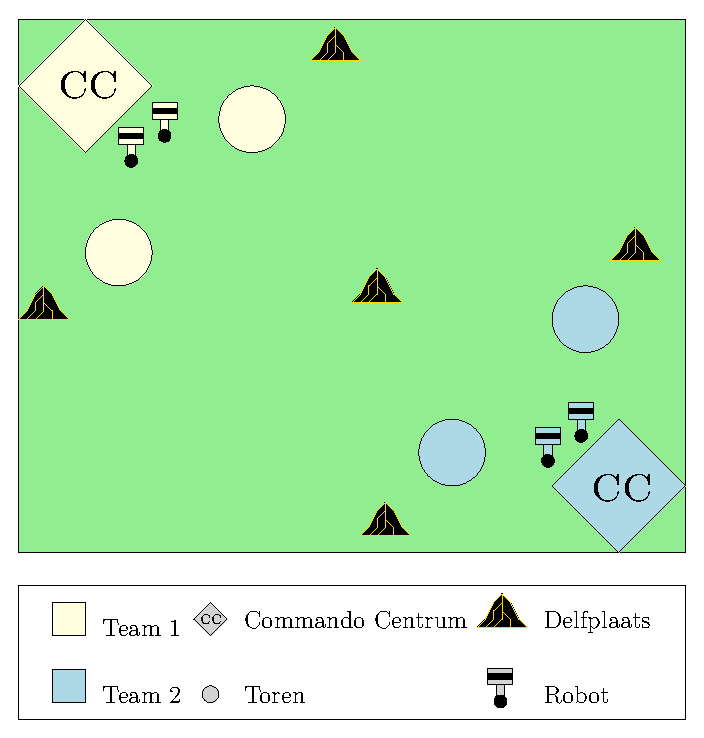
\includegraphics[width=\textwidth]{../Graphics/Map1.eps}
            \caption{Een bijna vierkant terrein met vier spelers}
            \label{fig:map1}
        \end{subfigure}\hspace{10mm}
        \begin{subfigure}{0.5\textwidth}
                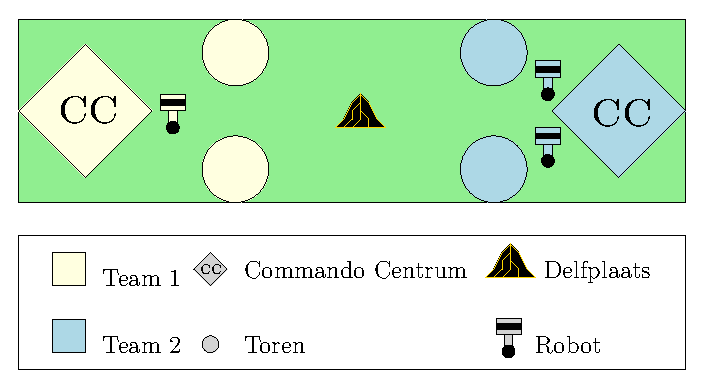
\includegraphics[width=\textwidth]{../Graphics/Map2.eps}
                \caption{Een breed terrein met drie spelers}
                \label{fig:map2}
        \end{subfigure}
        \caption{Twee verschillende beginconfiguraties van het spel}
    \end{figure}

    \subsection{Spelers}
    Een speler behoort tot \'e\'en van beide teams, spelers van een bepaald team zijn te identificeren door kleuren. De speler ziet de wereld vanuit de positie van zijn robot. Men kan de kijkrichting aanpassen, zodat deze elke willekeurige richting kan zijn. Als de kijkrichting verder naar links of rechts wordt gedraaid, draait de robot mee. De speler heeft een lasergeweer waarmee hij op andere spelers en torens kan schieten om deze te vernietigen. Het lasergeweer schiet laserstralen met een `oneindige' snelheid in de huidige kijkrichting. Bij het begin van het spel heeft de robot nog een volledig harnas. Zodra de speler wordt geraakt, wordt de conditie van het harnas slechter. Het is echter niet mogelijk dat een speler het harnas van een andere speler uit hetzelfde team beschadigt.
    \FloatBarrier
    Een speler gaat dood als zijn harnas kapot is. In dat geval zal hij na een bepaalde hoeveelheid tijd terugkeren bij het commandocentrum met een volledig harnas. Ook kan een speler gebouwen bouwen, hiervoor gebruikt hij goud uit de kas van het team. De spelers kunnen op het grondvlak bewegen met een vaste snelheid in elke richting. De enige voorwaarde hierbij is dat de spelers op de kaart blijven en niet door een gebouw lopen. Het is dus wel mogelijk dat spelers door elkaar heen kunnen lopen. De speler kijkt vanuit een derde persoon perspectief. In een derde persoon perspectief wordt de sc\`ene bekeken vanaf een punt vlak achter de speler. Het is eventueel mogelijk om dit verder uit te breiden, zodat de speler kan wisselen van derde persoon perspectief naar eerste persoon perspectief.

    \subsection{Gebouwen}
    Er zijn drie soorten gebouwen: torens, mijnen en commandocentra. Torens schieten op spelers en andere gebouwen in hun bereik. Mijnen kunnen over delfplaatsen worden gebouwd met het doel de inkomsten van een team te vergroten. In principe levert elke mijn een vaste hoeveelheid goud voor de gezamenlijke kas op. Deze hoeveelheid wordt periodiek toegevoegd aan de kas.

    Uit sommige delfplaatsen kan maar een bepaalde hoeveelheid goud worden gehaald, daarna is de delfplaats op. Dan zal de mijn over die delfplaats geen verdere bijdrage meer leveren voor de gezamenlijke kas. We staan echter ook delfplaatsen toe die een onbeperkte hoeveelheid goud bevatten. Standaard levert elke mijn hetzelfde bedrag op met dezelfde periode, maar dit kan later nog worden aangepast.

    Het commandocentrum is het belangrijkste gebouw van het team. Als dit gebouw kapot is, heeft het bijbehorende team verloren. Gebouwen kunnen door spelers worden beschoten, waardoor deze worden beschadigd. Gebouwen kunnen op geen enkele mogelijke manier hersteld worden. Optioneel zou men mechanismen in het spel kunnen toevoegen om deze gebouwen te herstellen. Alle gebouwen behoren tot \'e\'en van beide teams, deze gebouwen kunnen weer ge\"identificeerd worden door de kleur van het gebouw.

    \subsection{Verzamelbare voorwerpen}
    Er is maar \'e\'en verzamelbaar voorwerp: een muntje. E\'en of meerdere muntjes worden achtergelaten door spelers die dood gaan en torens die worden vernietigd. Een muntje heeft een bepaalde waarde in goud. De waarde van de muntjes zijn proportioneel aan de gezamenlijke kas van het team waarvan de speler is doodgegaan. Als een toren is vernietigd, dan is de waarde van de muntjes proportioneel aan de kosten van de toren. De waarde van de muntjes moet echter altijd kleiner zijn dan de kosten van de toren. Gedurende een spel moeten deze proporties vast zijn.

    Als een speler doodgaat, wordt bovendien nog de waarde van de muntjes afgetrokken van de gezamenlijke kas van die speler. Een muntje kan vervolgens opgepakt worden door alle spelers. Het muntje is dus het voedsel element in ons spel. De waarde van het muntje zal dan toegevoegd worden aan de kas van het bijbehorende team.

    \subsection{Initialisatie}
    De spelers kunnen zelf kiezen bij welk team ze gaan, onder de voorwaarde dat elk team minstens \'e\'en speler heeft. Bij de start van het spel staan alle spelers bij het commandocentrum. Zoals al eerder gezegd, hebben alle spelers dan nog een volledig harnas. Bovendien heeft elk team een zekere positieve hoeveelheid goud in de gezamenlijke kas, die voor beide teams natuurlijk gelijk moet zijn. Er kan minstens \'e\'en mijn gebouwd worden met deze hoeveelheid goud.
    \FloatBarrier

    \subsection{Gebruikersomgeving}
    \label{sec:UI}

    Via de gebruikersomgeving kan de speler de interactie met het 3D-model aangaan. De volgende componenten worden weergegeven op de gebruikersomgeving tijdens het spel:
    \begin{itemize}
    \item De hoeveelheid goud van het team, deze hoeveelheid staat achter een goudstaaf.
    \item De sterkte van het harnas, die wordt weergegeven door middel van een statusbalk.
    \item Het vizier van de speler.
    \item Een plattegrond.
    \end{itemize}

    We plaatsen het vizier van de speler altijd in het midden van het scherm. Hierdoor weet de speler dus in welke richting wordt geschoten. Voor de duidelijkheid hebben wij hier ook een figuur van gemaakt, zie figuur \ref{fig:UI}.
    \begin{figure}[H]
    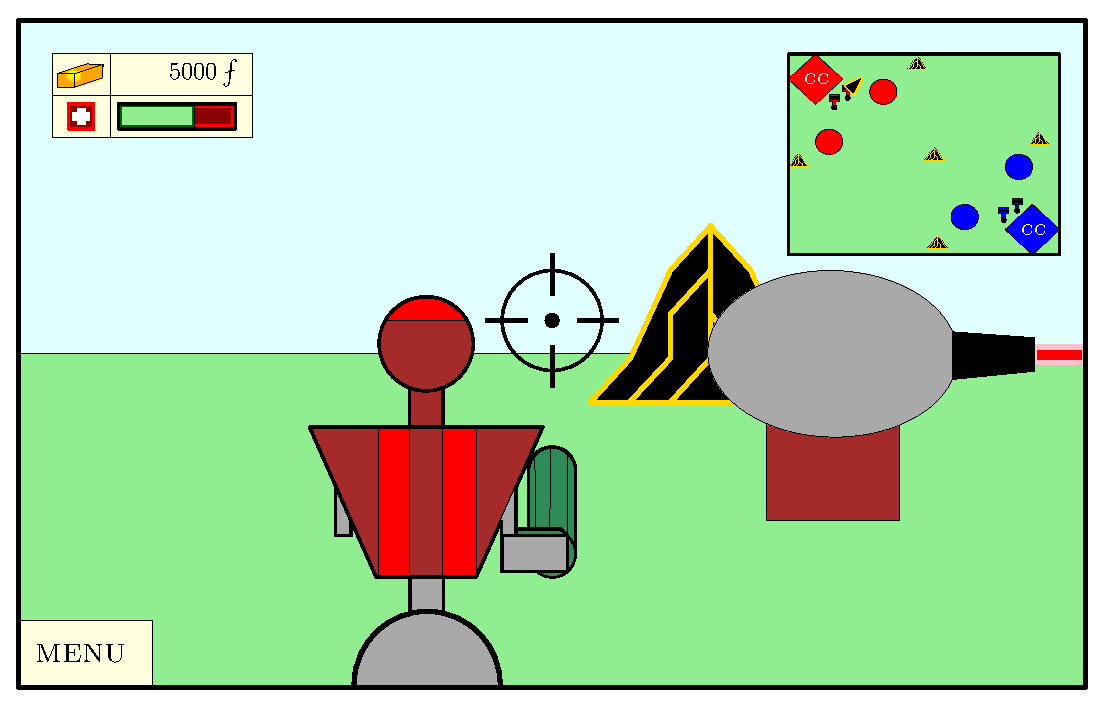
\includegraphics[width=0.9\textwidth]{../Graphics/UI.eps}
    \caption{De gebruikersomgeving tijdens het spel}
    \label{fig:UI}
    \end{figure}
    De besturing van de robot kan met de \textsc{wasd}-toetsencombinatie of door gebruik te maken van de pijltjes-toetsen. Hiervoor geven we de volgende tabel:
    \begin{table}[H]
        \small
        \centering
        \begin{tabular}{| l | l |}
        \hline
        Knop & Reactie \\ \hline
        \textsc{w} of $\uparrow$ & De robot beweegt, indien mogelijk, vooruit naar de huidige kijkrichting toe \\ \hline
        \textsc{a} of $\leftarrow$ & De robot draait naar links \\ \hline
        \textsc{s} of $\downarrow$ & De robot beweegt, indien mogelijk, achteruit van de huidige kijkrichting af \\ \hline
        \textsc{d} of $\rightarrow$ & De robot draait naar rechts \\ \hline
        \end{tabular}
        \caption{Knoppen met bijbehorende reactie}
        \label{tab:planning}
    \end{table}

    De speler kan schieten door op de muis te drukken. Een gedetailleerde beschrijving van het schieten is opgenomen in appendix \ref{app:schieten}. Door de muis naar boven of naar beneden te bewegen, kijkt de speler verder omhoog of omlaag respectievelijk. Op analoge wijze kan de speler naar links of naar rechts draaien door respectievelijk de muis naar links of naar rechts te bewegen. Merk op dat het vizier altijd in het midden van het scherm blijft. De speler ziet dit dus doordat de horizon omlaag of omhoog schuift.

    \subsection{Het neerzetten van gebouwen}
    De speler kan ook opdracht geven om op een bepaalde plek een gebouw neer te laten zetten. Om een gebouw neer te zetten moet de speler eerst op de knop \textsc{b} drukken. Dan gaat de speler in de zogenaamde \emph{bouw-modus}. Er wordt dan op de ondergrond een rooster getekend. Door middel van het vizier kan de speler een plek op het rooster aanwijzen. De speler kan dan door te klikken de opdracht geven om het gebouw te plaatsen. Op dat moment wordt de bijbehorende hoeveelheid goud uit de gezamenlijke kas gehaald. Dit kan natuurlijk alleen als de speler voldoende goud heeft.

    Indien de speler niet genoeg goud heeft, dan zal er een waarschuwing worden gegeven. Het gebouw zal dan ook niet worden geplaatst. Als de speler wel genoeg goud heeft, zal het gebouw uit de grond verrijzen. Na het neerzetten van het gebouw blijft de speler in de bouw-modus. Door nogmaals op de knop \textsc{b} te drukken gaat de speler weer uit de bouw-modus. Dit kan gezien worden in figuur \ref{fig:gebouw}.
    \begin{figure}
    \centering
    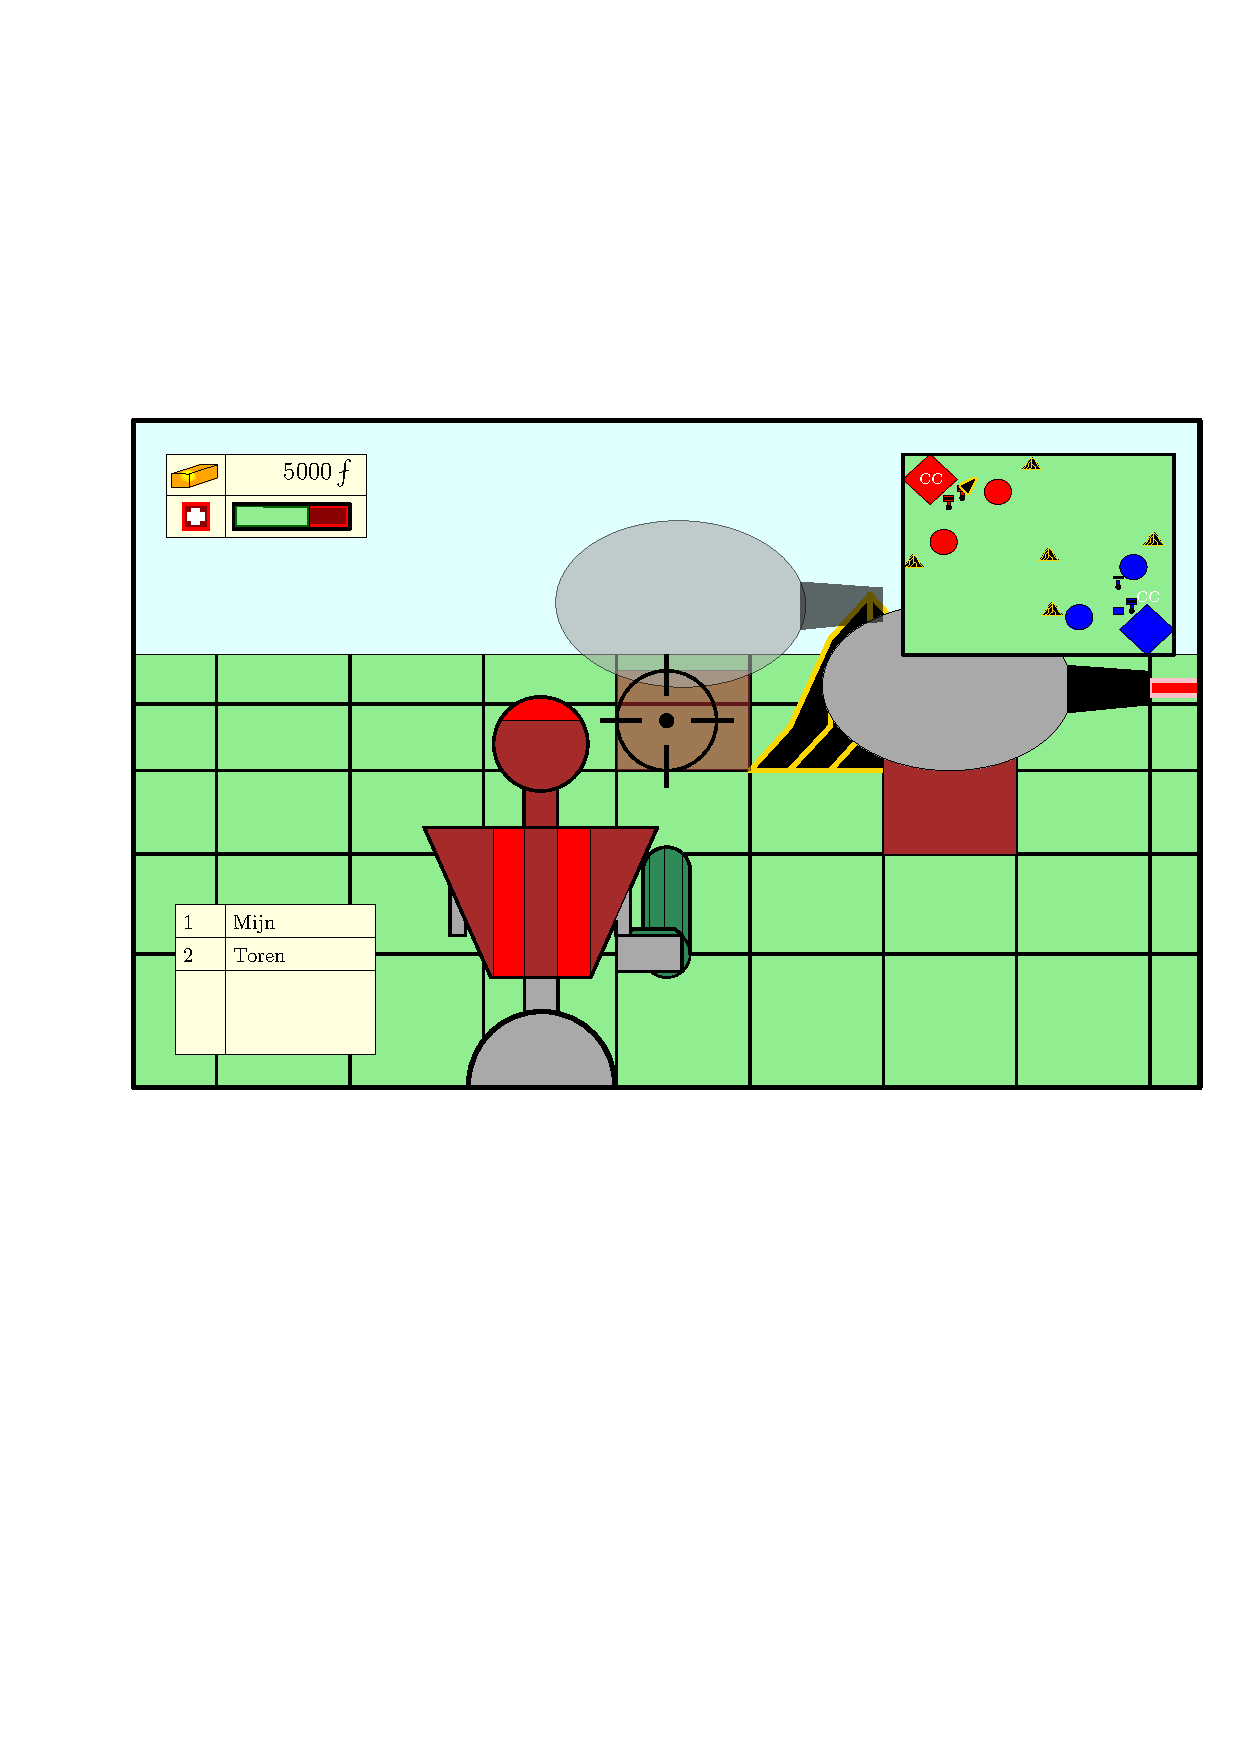
\includegraphics[width=\textwidth]{../Graphics/UI2.pdf}
    \caption{Een voorbeeld van het neerzetten van een gebouw in de gebruikersomgeving}
    \label{fig:gebouw}
    \end{figure} 
        \section{Beschrijving alternatieven}
    \label{app:alternatieven}
    Hier beschrijven we de door ons bekeken alternatieve ontwerpen voor een spel. Tijdens het brainstormen zijn we eerst de mogelijkheden gaan afbakenen door te kijken naar een aantal genres. Hierbij hebben we vooral gekeken naar persoonlijke voorkeuren. Verder hebben we natuurlijk rekening gehouden met het feit dat het spel een `voedsel' aspect moet hebben en dat het voor meerdere spelers moet zijn. Dit gaf de volgende genres:
    \begin{enumerate}
    \item[i] Strategie.
    \item[ii] Racen.
    \item[iii] First-Person Shooter.
    \item[iv] Levenssimulatie.
    \end{enumerate}
    We zullen nu elk genre dieper uitdiepen door de verschillende mogelijkheden verder in te vullen.

    \subsection{Strategie}
    We dachten bij strategie tijdens het brainstormen meteen aan het winnen van terrein als een vorm van `voedsel'. Het doel is dan om zoveel mogelijk terrein te winnen. Terrein wordt veroverd door een bepaalde tijd op een vakje te blijven staan. Verder dachten we al snel aan RTS, real-time strategie. Het idee is hier om `voedsel' te verzamelen om een leger te bouwen. Men wint dan door met dit leger de basis van de tegenstander te vernietigen.

    Via RTS kwamen we op het idee van \emph{Tower Defense}. Tower Defense wordt normaal gesproken met \'e\'en speler gespeeld. Vijandige monsters moeten dan worden tegen gehouden door torens te bouwen, die deze monsters voor jou aanvallen.

    \subsection{Racen}
    Bij een racespel dachten we aan twee alternatieven. De eerste optie was om het spelconcept van \emph{Mario Kart} ruwweg te volgen. Het doel hierbij is om zo snel mogelijk een vooraf vastgesteld aantal rondjes te rijden over een baan. Tijdens het rijden kunnen spelers power-ups verzamelen. De power-ups spelen hier dus de rol van het `voedsel'. Deze power-ups kunnen dan gebruikt worden om een voordeel te krijgen over andere spelers. Dit voordeel zou op zeer veel manieren kunnen worden gerealiseerd: zo zou een speler tijdelijk sneller kunnen gaan als gevolg van een power-up. Een andere mogelijkheid is de power-up af te kunnen schieten op andere spelers. Geraakte spelers kunnen dan worden vertraagd of tijdelijk stil komen te staan.

    Een tweede optie is dat spelers rond kunnen rijden in een grote stad. Het doel is dan om de auto's van alle andere spelers te vernietigen. Een auto van een tegenstander kan worden beschadigd door tegen de zijkant aan te rijden. Bovendien kan het spel verder worden uitgebreid, zodat de auto ook kan worden beschadigd door andere objecten.

    \subsection{First-Person Shooter}
    De First-Person Shooter is een alom bekend spelconcept. Een speler kan vrij over een gebied rondlopen. Meestal zal de speler een of ander wapen bij zich hebben. Met dit wapen kunnen andere spelers worden aangevallen. Het doel is dan om zoveel mogelijk medespelers uit te schakelen. Vaak is het zo dat een speler na een bepaalde tijd kan terugkeren in het spel, nadat die is uitgeschakeld.

    \subsection{Levenssimulatie}
    We dachten bij levenssimulatie aan een spel dat ge\"inspireerd is op het bekende spel \emph{Spore}. Ieder speler heeft in dit spel zijn eigen schepsel. Men kan zijn eigen schepsel laten groeien door andere schepsels, die niet noodzakelijk worden bestuurd door medespelers, op te eten. Het doel is dan om als enige over te blijven.

    \newpage
    \section{Motivering keuze}
    \label{app:motivering}
    In deze appendix motiveren we onze keuze uit de verschillende alternatieven in appendix \ref{app:alternatieven}. Tijdens het brainstormen was strategie meteen een van onze persoonlijke voorkeuren. Dit vonden wij allen een aantrekkelijk genre om te spelen. Het nadeel bij het veroveren van terrein is dat men al snel vastzit aan een grid. Dit is echter slechts een zeer kleine beperking. E\'en van onze verdere uitwerkingen van het genre strategie was RTS. Echter, RTS wordt al snel zeer complex om te maken, wat een groot nadeel is.

    Dit is ook de voornaamste reden dat we het simpelere Tower Defense hebben bekeken. Tower Defense is in onze mening relatief eenvoudig, maar toch aantrekkelijk om te spelen. De vraag was toen hoe Tower Defense kon worden uitgebreid tot een spel voor meerdere spelers. Het idee, dat hieruit kwam, is de basis voor het uiteindelijke spel, waarvan een korte samenvatting is uitgewerkt in het volgende hoofdstuk.

    Een racespel was ons voornaamste alternatief voor strategie. Ook dit vonden wij allen een aantrekkelijk genre om te spelen. We hadden hier, zoals al eerder besproken, ruwweg twee idee\"en: bij de eerste optie was het doel om zo snel mogelijk een vooraf bepaald aantal rondjes te rijden, bij de tweede optie was het doel om de auto's van alle andere spelers te vernietigen.

    Bij de eerste optie is er een mogelijk probleem dat power-ups, die in onze mening vitaal zijn om het spel leuk te maken, niet makkelijk kunnen worden ge\"implementeerd. Er zijn drie potenti\"ele problemen bij de tweede optie: zo is het niet duidelijk wat het `voedsel' aspect hier is. Bovendien is het zeker niet eenvoudig om te bepalen wie tegen wie aanrijdt. Als laatste is het visueel weergeven van de schade aan een auto lastig.

    Het spelconcept van First-Person Shooter hebben we niet uitgebreid bekeken tijdens het brainstormen. Ons voornaamste bezwaar was dat het zeer gecompliceerd is om te bepalen of iemand is geraakt door een kogel. Aangezien dit een zeer complex spelconcept is, willen wij dit zo simpel mogelijk houden. Daarom hebben we besloten dat spelers elkaar beschieten met lasers, die een snelheid van `oneindig' hebben. Zo kan dus direct bij het schot worden bepaald of het raak dan wel niet raak is. Dit vermijdt het probleem van bewegende objecten in de scene.

    Een groot voordeel is dat First-Person Shooters uit zichzelf al voor meerdere spelers zijn. Daarom is een deel van het First-Person Shooter concept ook opgenomen in het uiteindelijke spelconcept. Op deze manier kon het Tower Defense concept verder worden aangevuld tot een spel voor meerdere spelers: spelers kunnen elkaar aanvallen in het spel door elkaar te beschieten.

    Bij het idee van levenssimulatie werden wij ge\"inspireerd door het welbekende Spore, wat door een aantal van ons met enthousiasme is gespeeld. Er is ook een zeer duidelijk `voedsel' aspect aanwezig. Het was ons echter niet duidelijk hoe dit spel op een aantrekkelijke doch eenvoudige manier kon worden uitgebreid naar een spel voor meerdere spelers.

    \subsection{Het spel}
    Het uiteindelijke spel combineert een aantal van de eerdere idee\"en, met name Tower Defense en First-Person Shooter. We geven hier slechts een korte samenvatting van het spel. Een uitgebreide beschrijving van het spel staat in de spelspecificatie. We verdelen de spelers in twee teams. Spelers kunnen over het terrein rondlopen. Terwijl spelers rondlopen, kunnen ze torens bouwen met goud. Er zijn twee type torens: het eerste type toren kan op een mijn worden gebouwd en verzamelt extra goud. Het tweede type toren kan spelers aanvallen. Spelers kunnen andere spelers en torens aanvallen, dit is meteen ook de tweede manier om goud te verdienen. Als spelers doodgaan, komen ze een tijd later weer bij een speciaal gebouw terecht: het hoofdgebouw. Elk team heeft ook een hoofdgebouw, het doel van het spel is om het hoofdgebouw van het andere team te vernietigen.

    We hebben dus uiteindelijk gekozen voor een combinatie van de eerder genoemde spelconcepten. In onze mening is het daarmee een potentieel aantrekkelijk en innovatief spel. Het innovatieve element aan het spel is dat zowel elementen uit RTS als First-Person Shooter worden gecombineerd. Het grootste probleem is echter daarmee meteen de haalbaarheid van het spel. Elk spel moet al rekening houden met het netwerk aspect en bovendien met het gedistribueerde aspect, aangezien er geen server mag zijn tijdens het spel.  
    % Reference berichten
    % Appendices in ontwerp verkeerde REFERENCE
        \section{Het ontwerp}
    % Inclusief alternatieven, motivering van keuzes, aannames en communicatieprotocol
    Nu zijn we klaar om het ontwerp van ons spel \textsc{GOTO} te bespreken. We zullen beginnen door de verschillende componenten te analyseren. Het programma is hierbij verdeeld in drie zo onafhankelijk mogelijke componenten. Wij onderscheiden de volgende componenten:
    \begin{itemize}
    \item Een component die het communiceren naar andere spelers mogelijk maakt;
	\item Het model van de sc\`ene. Denk hierbij aan de staat, locatie en grafische modellen van gebouwen, spelers en het terrein;
	\item De gebruikersomgeving die de interactie van de speler met het spel mogelijk maakt en ook het grafische model weergeeft tijdens het spel.
    \end{itemize}

    Als uitgangspunt ontwerpen wij de verschillende componenten zodanig dat elke component zo onafhankelijk mogelijk ontwikkeld kan worden.
    	
    \subsection{Protocol module}
    De protocol module is het onderdeel die het mogelijk maakt om:
	\begin{itemize}
    \item Een nieuw spel op te starten. Het spel komt dan in de zogenaamde opstart fase. Andere spelers kunnen dan aan dit spel meedoen, ze komen dan in de lobby van dat spel;
	\item De lijst van alle spellen, die nog in de opstart fase zijn, in het subnet van de computer weer te geven;
	\item Mee te doen met een bestaand spel dat nog in de opstart fase zit;
	\item Het spel te beginnen;
	\item Mutaties van de staat van het spel te ontvangen en te versturen.
	\end{itemize}
    De manier, waarop deze communicatie verloopt, is beschreven vanaf \protoref. De gebruikersomgeving kan de protocol module een opdracht geven. Deze    opdracht zal dan asynchroon worden uitgevoerd door de protocol module. Dit betekent dat het protocol uit zichzelf berichten kan ontvangen en verwerken. Door middel van threads wordt er voor gezorgd dat het protocol de taken onafhankelijk kan uitvoeren.
	
    \subsection{Het model van de sc\`ene}
    Het model van de sc\`ene vervult twee rollen. Het houdt de huidige staat van het spel bij en zorgt ervoor dat de huidige staat van het spel afgebeeld kan worden op het scherm. Het model is dus in principe een passief element, het zal niet uit zichzelf acties uitvoeren (uitzonderingen daargelaten). Een diepgaande beschrijving van het model kan gevonden worden in appendix \ref{app:klassenbeschrijving}.

    \subsection{Gebruikersomgeving}
    De gebruikersomgeving moet zowel het grafische model van het spel afbeelden op het scherm als de interactie van de speler via het toetsenbord en muis afhandelen. Ook moet de gebruikersomgeving het mogelijk maken voor de gebruiker om een spel op te starten of mee te doen aan een spel in de opstart fase.

    \subsubsection{De opzet van het spel}
    Tijdens de opzet van het spel zal de gebruikersomgeving een venster weer moeten geven met alle spellen in het subnet van de computer. De gebruiker kan dan kiezen om mee te doen aan een van deze spellen of zijn eigen spel te openen. Als de gebruiker zelf een spel opent, kunnen andere gebruikers in hetzelfde subnet ook meedoen aan dit spel. Deze spelers kunnen dan met elkaar communiceren in een lobby. Hierin kunnen zij ook aangeven of zij klaar zijn om het spel te starten. Zodra alle gebruikers hebben aangegeven dat zij klaar zijn, kan het spel worden gestart. De keuze om het spel te starten is dan aan de gebruiker, die ook het spel heeft geopend.

    \subsubsection{Tijdens het spel}
    De gebruikersomgeving zal tijdens het spel via \textsc{openGL} de lokale staat van het spel afbeelden op het scherm. Dit wordt gedaan door de \emph{render} methode van het object \emph{World} aan te roepen, die is beschreven in sectie \ref{sec:model}. De gebruikersomgeving zal daarna alleen nog menu's, mogelijke kaarten en informatie als de sterkte van het harnas en de hoeveelheid geld op het scherm moeten aangeven (zoals beschreven in het document Informele Beschrijving). Door de 2D-modus van openGL te gebruiken kan dit gemakkelijk getekend worden boven op de grafische representatie van de wereld.

    De gebruikersomgeving zal ook het model aanpassen aan de hand van de interactie van de gebruiker met de omgeving. Om dit voor elkaar te krijgen slaat
    de gebruikersomgeving alle muisbewegingen, klikken en toetsenbord aanslagen op en past het model op de bijbehorende manier aan. Een verdere uitleg van de interactie tussen de gebruikersomgeving en het model is gegeven in sectie \ref{sec:interactie}.

    \section{Onderlinge samenhang}
    \label{sec:protocol}
    De drie onderdelen, die wij hierboven beschreven hebben, moeten natuurlijk allemaal met elkaar kunnen communiceren. Deze communicatie zullen we nu beschrijven.

    \subsection{Gebruikersomgeving en protocol module tijdens de opzet van het spel}
    De gebruikersomgeving en de protocol module communiceren tijdens de opzet van het spel compleet asymmetrisch. Dat wil zeggen dat het protocol op elk moment een bericht kan sturen naar de gebruikersomgeving en ook andersom. Om dit mogelijk te maken, heeft de protocol module verschillende functies ge\"implementeerd, die aangeroepen kunnen worden door de gebruikersomgeving. Deze kunnen bijvoorbeeld gebruikt worden om een nieuw spel aan te maken of mee te doen aan een bestaand spel. Op deze manier kan de gebruikersomgeving acties van de gebruiker omzetten in een actie van het protocol: de protocol module handelt dit dan af.

    De protocol module luistert actief naar binnenkomende berichten. Aangezien het protocol real-time verplichtingen heeft, zal de module gebruik maken van meerdere threads. Zo fungeert de module los van de gebruikersomgeving. Als er een bijzondere gebeurtenis heeft plaatsgevonden, kan het protocol dit doorgeven aan de gebruikersomgeving door middel van zogenaamde \emph{call-backs}. Dit zijn methoden die de gebruikersomgeving implementeert, zodat de protocol module informatie kan doorgeven aan de gebruikersomgeving. De gebruikersomgeving zal deze informatie zodanig moeten afhandelen dat het afgebeeld kan worden op het scherm.

    Niet alle communicatie van de protocol module en de gebruikersomgeving verloopt via call-backs en methoden, sommige informatie zal de protocol module namelijk niet als een gebeurtenis doorgeven. Deze informatie wordt louter opgeslagen in de protocol module en kan de gebruikersomgeving opvragen. Denk hierbij aan de lijst van spellen op het subnet, spelers in het spel, enzovoorts. Een voorbeeld van interactie van de gebruikersomgeving en protocol module is gegeven in een \textsc{msc} in appendix \ref{app:MSCLobbyCon}.

    \subsection{Model van de sc\`ene en de gebruikersomgeving tijdens het spel}
    \label{sec:interactie}
    Het model van de sc\`ene zal niet actief communiceren met de gebruikersomgeving tijdens het spel. Dat wil zeggen dat er geen asymmetrische communicatie plaatsvindt via call-backs. De gebruikersomgeving zal aan de hand van de invoer van de gebruiker het model aanpassen. De gebruikersomgeving zal ook de grafische representatie van de staat van het spel uit het model halen. Het model maakt dit mogelijk door de beschreven \emph{render} methode in de interface \emph{object}. Het model zorgt voor enkele globale methoden die in \'e\'en keer een actie van de gebruiker kan verwerken in het model. Hierdoor hoeft de gebruikersomgeving alleen een paar globale methoden aan te roepen. Hiermee voorkomen wij dat de gebruikersomgeving veel gebruik moet maken van de structuur van het model. Zo wordt de gebruikersomgeving minder afhankelijk van de implementatie van het model.

    We hebben nu de verschillende componenten en hun onderlinge communicatie uitgediept. Een volledige beschrijving van de klassen wordt gegeven in appendix \ref{app:klassenbeschrijving}. Er is ook een bijbehorend klassediagram gemaakt. Het klassediagram is te vinden in appendix \ref{app:klassendiagram}. We zullen nu verder gaan met de beschrijving van het protocol.

    \section{De opbouw van de graaf}
    Het protocol zal een volledige graaf proberen op te bouwen. Het berichtsformaat wordt formeel gedefinieerd in appendix \ref{app:berichtsformaat}. De bijbehorende berichten zijn beschreven in appendix \ref{app:berichten}. Dit wordt gedaan tijdens de lobby fase van het spel. We weten dat er tijdens de lobby fase een server is. Elk proces probeert nu een \tcp-connectie te maken met deze server. Zodra deze \tcp-connectie is geslaagd, zal het proces een lijst teruggestuurd krijgen. Deze lijst bevat alle adressen van processen, waarmee de server nu is verbonden. Verbindingen uit de lobby fase tellen hierbij dus niet mee. Het proces is dan zelf verantwoordelijk om een \tcp-connectie aan te gaan met elk proces in deze lijst.

    Dit betekent dat op elk willekeurig moment een aanvraag voor een \tcp-connectie kan binnenkomen bij processen, die al een \tcp-connectie met de server hebben. Kortom, elk proces zal regelmatig moeten controleren op aanvragen voor een \tcp-connectie. Als de volledige graaf is opgebouwd, staan alle processen op gelijke voet. Op dat moment kan het spel beginnen.

    \section{Het protocol tijdens het spel}
    \label{sec:tijdensspel}
    De staat van het spel wordt uniek vastgelegd door de waarde van alle variabelen, inclusief de toestand van alle \tcp-connecties. Het is echter ondoenlijk om alle waarden van de variabelen voortdurend te versturen over de \tcp-connecties. Daarom zal elke speler een replica van het spel hebben. Deze replica's moeten natuurlijk zodanig worden gesynchroniseerd dat spelers er niet achterkomen dat hun replica's op kleine details tijdelijk kunnen verschillen.

    \subsection{Reliable en unreliable variabelen}
    We maken daarom onderscheid tussen twee soorten variabelen, \emph{reliable} en \emph{unreliable}. Reliable variabelen moeten gelijk zijn voor alle replica's om inconsistentie te voorkomen. Unreliable variabelen mogen wel verschillen tussen de spelers. Deze kunnen dus worden `gesimuleerd' door spelers. Om de reliable variabelen consistent te houden hebben we zogenaamde \emph{mutual exclusion} nodig. Een goed voorbeeld hiervan is het oprapen van een muntje.

    We pakken dit probleem aan door de notie van autoriteit te introduceren. Op elk moment heeft precies \'e\'en proces autoriteit. Als het proces autoriteit heeft, dan mag het proces reliable variabelen veranderen. Hiervoor wordt een bericht naar elk ander proces gestuurd. Het proces wacht dan totdat iedereen heeft teruggestuurd dat dit bericht is ontvangen. Als het proces alle wijzigingen van reliable variabelen heeft doorgegeven, krijgt een ander proces autoriteit.

    \subsection{De token ring}
    De volgende vraag is nu hoe we deze notie van autoriteit gaan verwerken in het protocol. Dit doen we door gebruik te maken van een \emph{token ring}. We bouwen tijdens de lobby fase (opstart fase) ook een ring op tussen alle processen. Dit doen we pas nadat de volledige graaf al is opgebouwd. Een mogelijke aanpak om dan een ring op te bouwen is om aan ieder proces een verschillend element uit een totaal geordend domein toe te kennen.

    We kunnen dit beschouwen als een injectieve functie $f$ van de verzameling processen $P$ naar een totaal geordende domein. Aangezien er sprake is van een totaal geordend domein, kunnen we deze waarden sorteren. Stel nu dat $P = \{ p_1, \ldots p_n\}$. Dit geeft ons een permutatie $\sigma$ zodanig dat:
    \[
    f(p_{\sigma(1)}) < f(p_{\sigma(2)}) < \ldots < f(p_{\sigma(n)})
    \]
    We verbinden nu $p_{\sigma(1)}$ met $p_{\sigma(2)}$, $p_{\sigma(2)}$ met $p_{\sigma(3)}$ enzovoorts. Bovendien verbinden we $p_{\sigma(n)}$ met $p_{\sigma(1)}$. We zijn er nu dus in geslaagd om de ring te construeren. Voor het totaal geordende domein kunnen we IP-adressen gebruiken, zodat uniciteit is gegarandeerd.

    Zodra een proces het token heeft, heeft het proces autoriteit. Het kan dan alle gewenste veranderingen van de reliable variabelen doorsturen over de volledige graaf. De andere processen zullen dan een \emph{acknowledgement} terugsturen dat dit bericht is ontvangen. Zodra alle acknowledgements van de andere processen zijn ontvangen, zal het proces de token zo snel mogelijk doorsturen naar het volgende proces in de ring. Dit zorgt ervoor dat elk proces binnen een eindige hoeveelheid tijd de token krijgt. Er is dus een zekere vorm van \emph{fairness}.

    \subsection{Simulatie}
    Sommige acties mogen ook worden uitgevoerd wanneer het desbetreffende proces niet de token heeft. Een speler mag bijvoorbeeld vrij rondlopen zonder dit te vragen aan alle andere spelers. Dit kan ervoor zorgen dat niet alle processen exact dezelfde staat hebben. Het is echter voldoende als alle processen naar dezelfde staat convergeren. We zullen dit verder toelichten aan de hand van een voorbeeld.

    Een proces zal de positie van alle andere spelers simuleren. Dit wordt gedaan met behulp van de locatie en de looprichting. De actuele locatie en looprichting van de desbetreffende speler zal periodiek over de volledige graaf worden verstuurd. Om eventuele problemen te voorkomen zou deze periode redelijk klein moeten zijn. In de tussentijd zal het proces de huidige locatie en looprichting van de speler benaderen door de speler simpelweg `verder' te laten lopen. Merk op dat op deze manier de speler ten alle tijden de baas blijft over zijn eigen locatie.

    \section{Aannamen}
    We hebben al eerder genoemd dat het \emph{Broadcast} bericht over \udp wordt gestuurd. Hier gebruiken we de broadcast functionaliteit van \udp voor. Het is dus noodzakelijk dat alle spelers zich op hetzelfde subnet bevinden. We weten dat \udp-berichten niet noodzakelijk aan hoeven te komen. We nemen echter aan dat een \udp-bericht uiteindelijk wordt ontvangen binnen een eindige hoeveelheid tijd, als de server periodiek \udp-berichten blijft versturen.

    Een speler kan dan een keuze maken tussen alle servers, waarvan een \emph{Broadcast} bericht is ontvangen. De speler gaat dan een \tcp-connectie aan met de uitgekozen server. We nemen aan dat deze \tcp-connectie succesvol wordt aangemaakt. Bovendien nemen we aan dat \tcp inderdaad voldoet aan de FIFO-eigenschap. Verder nemen we aan dat berichten over \tcp ook aankomen, eventueel nadat dit bericht een aantal keer opnieuw is verstuurd.

    Verder maken we nog een aantal simpele aannamen over de snelheid van het netwerk en de computers. De gebruikte berichten zijn allemaal zeer klein. We verwachten daarom dat er elke seconde zonder problemen 300 berichten over het netwerk kunnen worden verstuurd. Dit zou ruim voldoende moeten zijn om de replica's goede benaderingen van de werkelijke staat te laten zijn. Hiermee bedoelen we met een goede benadering dat het verschil met de werkelijke staat niet zou moeten opvallen voor de spelers.

    De helft van de RTT, oftewel de \emph{Round-Trip Time}, is een goede benadering voor hoe lang het duurt om een bericht te versturen. We gaan ervan uit dat de RTT kleiner is dan 200 ms. Deze aanname is zeker realistisch, aangezien de spelers in principe op hetzelfde subnet zitten. Vanwege deze aanname krijgen we ook een harde grens op de maximale afwijking van de replica's.
    \label{app:MSCLobbyCon} 

    \section{Conclusie}
    % Met daarin reflectie over het verloop van het project en het groepsproces daarbij

    \section{Evaluatie}
    % Wat is bereikt
    % Hoe het project is verlopen

    \section{Literatuurlijst}

    \newpage
    \appendix
    \section{Begrippenlijst}
    % Andere appendices

\end{document} 